\scalebox{0.7}{
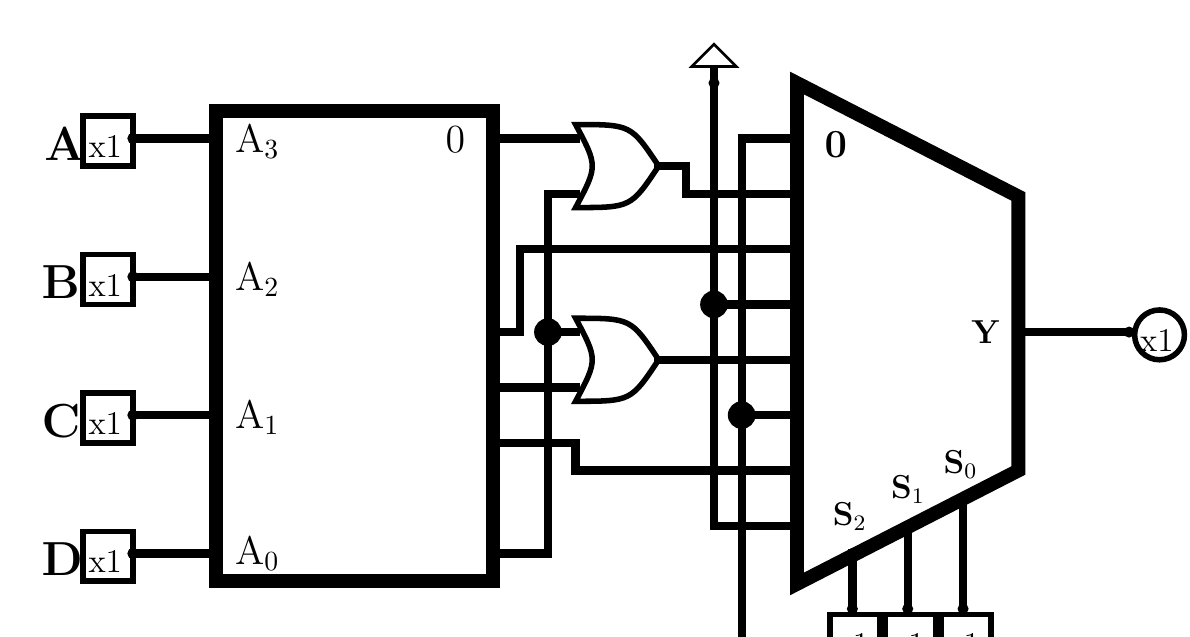
\begin{tikzpicture}[x=1pt,y=-1pt,line cap=rect]
\useasboundingbox (0,0) rectangle (410,210);
\def\logisimfontA#1{\fontfamily{cmr}{#1}} % Replaced by logisim, original font was "SansSerif"
\def\logisimfontB#1{\fontfamily{Lexend}{#1}}
\definecolor{custcol_0_0_0}{RGB}{0, 0, 0}
\definecolor{custcol_ff_ff_ff}{RGB}{255, 255, 255}
\draw [line width=3.0pt, custcol_0_0_0 ]  (228.0,120.0) -- (278.0,120.0) ;
\draw [line width=3.0pt, custcol_0_0_0 ]  (358.0,110.0) -- (398.0,110.0) ;
\draw [line width=3.0pt, custcol_0_0_0 ]  (298.0,190.0) -- (298.0,210.0) ;
\draw [line width=3.0pt, custcol_0_0_0 ]  (318.0,180.0) -- (318.0,210.0) ;
\draw [line width=3.0pt, custcol_0_0_0 ]  (338.0,170.0) -- (338.0,210.0) ;
\draw [line width=3.0pt, custcol_0_0_0 ]  (38.0,40.0) -- (68.0,40.0) ;
\draw [line width=3.0pt, custcol_0_0_0 ]  (38.0,90.0) -- (68.0,90.0) ;
\draw [line width=3.0pt, custcol_0_0_0 ]  (38.0,140.0) -- (68.0,140.0) ;
\draw [line width=3.0pt, custcol_0_0_0 ]  (38.0,190.0) -- (68.0,190.0) ;
\draw [line width=3.0pt, custcol_0_0_0 ]  (248.0,100.0) -- (278.0,100.0) ;
\draw [line width=3.0pt, custcol_0_0_0 ]  (258.0,140.0) -- (278.0,140.0) ;
\draw [line width=3.0pt, custcol_0_0_0 ]  (228.0,50.0) -- (238.0,50.0) -- (238.0,60.0) -- (278.0,60.0) ;
\draw [line width=3.0pt, custcol_0_0_0 ]  (168.0,110.0) -- (178.0,110.0) -- (178.0,80.0) -- (278.0,80.0) ;
\draw [line width=3.0pt, custcol_0_0_0 ]  (168.0,150.0) -- (198.0,150.0) -- (198.0,160.0) -- (278.0,160.0) ;
\fill [line width=3.0pt, custcol_0_0_0]  (248.0,100.0) ellipse (5.0 and 5.0 );
\fill [line width=3.0pt, custcol_0_0_0]  (188.0,110.0) ellipse (5.0 and 5.0 );
\fill [line width=3.0pt, custcol_0_0_0]  (258.0,140.0) ellipse (5.0 and 5.0 );
\draw [line width=2.0pt, custcol_0_0_0 ]  (20.0,32.0) -- (37.0,32.0) ;
\draw [line width=2.0pt, custcol_0_0_0 ]  (38.0,32.0) -- (38.0,49.0) ;
\draw [line width=2.0pt, custcol_0_0_0 ]  (38.0,50.0) -- (21.0,50.0) ;
\draw [line width=2.0pt, custcol_0_0_0 ]  (20.0,50.0) -- (20.0,33.0) ;
\logisimfontA{\fontsize{12pt}{12pt}\selectfont\node[inner sep=0, outer sep=0, custcol_0_0_0, anchor=base west] at  (22.0,47.0)  {x1};}
\logisimfontA{\fontsize{16pt}{16pt}\fontseries{bx}\selectfont\node[inner sep=0, outer sep=0, custcol_0_0_0, anchor=base west] at  (6.0,48.0)  {A};}
\fill [line width=2.0pt, custcol_0_0_0]  (38.0,40.0) ellipse (2.0 and 2.0 );
\draw [line width=2.0pt, custcol_0_0_0 ]  (20.0,82.0) -- (37.0,82.0) ;
\draw [line width=2.0pt, custcol_0_0_0 ]  (38.0,82.0) -- (38.0,99.0) ;
\draw [line width=2.0pt, custcol_0_0_0 ]  (38.0,100.0) -- (21.0,100.0) ;
\draw [line width=2.0pt, custcol_0_0_0 ]  (20.0,100.0) -- (20.0,83.0) ;
\logisimfontA{\fontsize{12pt}{12pt}\selectfont\node[inner sep=0, outer sep=0, custcol_0_0_0, anchor=base west] at  (22.0,97.0)  {x1};}
\logisimfontA{\fontsize{16pt}{16pt}\fontseries{bx}\selectfont\node[inner sep=0, outer sep=0, custcol_0_0_0, anchor=base west] at  (5.0,98.0)  {B};}
\fill [line width=2.0pt, custcol_0_0_0]  (38.0,90.0) ellipse (2.0 and 2.0 );
\draw [line width=2.0pt, custcol_0_0_0 ]  (20.0,132.0) -- (37.0,132.0) ;
\draw [line width=2.0pt, custcol_0_0_0 ]  (38.0,132.0) -- (38.0,149.0) ;
\draw [line width=2.0pt, custcol_0_0_0 ]  (38.0,150.0) -- (21.0,150.0) ;
\draw [line width=2.0pt, custcol_0_0_0 ]  (20.0,150.0) -- (20.0,133.0) ;
\logisimfontA{\fontsize{12pt}{12pt}\selectfont\node[inner sep=0, outer sep=0, custcol_0_0_0, anchor=base west] at  (22.0,147.0)  {x1};}
\logisimfontA{\fontsize{16pt}{16pt}\fontseries{bx}\selectfont\node[inner sep=0, outer sep=0, custcol_0_0_0, anchor=base west] at  (5.0,148.0)  {C};}
\fill [line width=2.0pt, custcol_0_0_0]  (38.0,140.0) ellipse (2.0 and 2.0 );
\draw [line width=2.0pt, custcol_0_0_0 ]  (20.0,182.0) -- (37.0,182.0) ;
\draw [line width=2.0pt, custcol_0_0_0 ]  (38.0,182.0) -- (38.0,199.0) ;
\draw [line width=2.0pt, custcol_0_0_0 ]  (38.0,200.0) -- (21.0,200.0) ;
\draw [line width=2.0pt, custcol_0_0_0 ]  (20.0,200.0) -- (20.0,183.0) ;
\logisimfontA{\fontsize{12pt}{12pt}\selectfont\node[inner sep=0, outer sep=0, custcol_0_0_0, anchor=base west] at  (22.0,197.0)  {x1};}
\logisimfontA{\fontsize{16pt}{16pt}\fontseries{bx}\selectfont\node[inner sep=0, outer sep=0, custcol_0_0_0, anchor=base west] at  (5.0,198.0)  {D};}
\fill [line width=2.0pt, custcol_0_0_0]  (38.0,190.0) ellipse (2.0 and 2.0 );
\draw [line width=3.0pt, custcol_0_0_0 ]  (278.0,180.0) -- (248.0,180.0) -- (248.0,100.0) -- (248.0,20.0) -- (248.0,15.0) ;
\draw [line width=1.0pt, custcol_0_0_0 ]  (240.0,14.0) -- (248.0,6.0) -- (256.0,14.0) -- cycle;
\fill [line width=1.0pt, custcol_0_0_0]  (248.0,20.0) ellipse (2.0 and 2.0 );
\draw [line width=3.0pt, custcol_0_0_0 ]  (278.0,40.0) -- (258.0,40.0) -- (258.0,140.0) -- (258.0,230.0) -- (258.0,235.0) ;
\draw [line width=1.0pt, custcol_0_0_0 ]  (266.0,236.0) -- (250.0,236.0) ;
\draw [line width=1.0pt, custcol_0_0_0 ]  (263.0,239.0) -- (253.0,239.0) ;
\draw [line width=1.0pt, custcol_0_0_0 ]  (260.0,242.0) -- (256.0,242.0) ;
\fill [line width=1.0pt, custcol_0_0_0]  (258.0,230.0) ellipse (2.0 and 2.0 );
\draw [line width=2.0pt, custcol_0_0_0 ]  (290.0,212.0) -- (307.0,212.0) ;
\draw [line width=2.0pt, custcol_0_0_0 ]  (308.0,212.0) -- (308.0,229.0) ;
\draw [line width=2.0pt, custcol_0_0_0 ]  (308.0,230.0) -- (291.0,230.0) ;
\draw [line width=2.0pt, custcol_0_0_0 ]  (290.0,230.0) -- (290.0,213.0) ;
\logisimfontA{\fontsize{12pt}{12pt}\selectfont\node[inner sep=0, outer sep=0, custcol_0_0_0, anchor=base west] at  (292.0,227.0)  {x1};}
\logisimfontA{\fontsize{16pt}{16pt}\fontseries{bx}\selectfont\node[inner sep=0, outer sep=0, custcol_0_0_0, anchor=base west] at  (293.0,249.0)  {E};}
\fill [line width=2.0pt, custcol_0_0_0]  (298.0,210.0) ellipse (2.0 and 2.0 );
\draw [line width=2.0pt, custcol_0_0_0 ]  (310.0,212.0) -- (327.0,212.0) ;
\draw [line width=2.0pt, custcol_0_0_0 ]  (328.0,212.0) -- (328.0,229.0) ;
\draw [line width=2.0pt, custcol_0_0_0 ]  (328.0,230.0) -- (311.0,230.0) ;
\draw [line width=2.0pt, custcol_0_0_0 ]  (310.0,230.0) -- (310.0,213.0) ;
\logisimfontA{\fontsize{12pt}{12pt}\selectfont\node[inner sep=0, outer sep=0, custcol_0_0_0, anchor=base west] at  (312.0,227.0)  {x1};}
\logisimfontA{\fontsize{16pt}{16pt}\fontseries{bx}\selectfont\node[inner sep=0, outer sep=0, custcol_0_0_0, anchor=base west] at  (313.0,249.0)  {F};}
\fill [line width=2.0pt, custcol_0_0_0]  (318.0,210.0) ellipse (2.0 and 2.0 );
\draw [line width=2.0pt, custcol_0_0_0 ]  (330.0,212.0) -- (347.0,212.0) ;
\draw [line width=2.0pt, custcol_0_0_0 ]  (348.0,212.0) -- (348.0,229.0) ;
\draw [line width=2.0pt, custcol_0_0_0 ]  (348.0,230.0) -- (331.0,230.0) ;
\draw [line width=2.0pt, custcol_0_0_0 ]  (330.0,230.0) -- (330.0,213.0) ;
\logisimfontA{\fontsize{12pt}{12pt}\selectfont\node[inner sep=0, outer sep=0, custcol_0_0_0, anchor=base west] at  (332.0,227.0)  {x1};}
\logisimfontA{\fontsize{16pt}{16pt}\fontseries{bx}\selectfont\node[inner sep=0, outer sep=0, custcol_0_0_0, anchor=base west] at  (332.0,249.0)  {G};}
\fill [line width=2.0pt, custcol_0_0_0]  (338.0,210.0) ellipse (2.0 and 2.0 );
\draw [line width=3.0pt, custcol_0_0_0 ]  (168.0,40.0) -- (198.0,40.0) -- (198.0,40.0) ;
\draw [line width=3.0pt, custcol_0_0_0 ]  (198.0,60.0) -- (198.0,60.0) -- (188.0,60.0) -- (188.0,110.0) ;
\draw [line width=2.0pt, custcol_0_0_0 ]  (228.0,50.0) .. controls  (218.0,35.0)  ..  (198.0,35.0) .. controls  (206.0,50.0)  ..  (198.0,65.0) .. controls  (218.0,65.0)  ..  (228.0,50.0) -- cycle ;
\draw [line width=3.0pt, custcol_0_0_0 ]  (168.0,190.0) -- (188.0,190.0) -- (188.0,110.0) -- (198.0,110.0) -- (198.0,110.0) ;
\draw [line width=3.0pt, custcol_0_0_0 ]  (168.0,130.0) -- (198.0,130.0) -- (198.0,130.0) ;
\draw [line width=2.0pt, custcol_0_0_0 ]  (228.0,120.0) .. controls  (218.0,105.0)  ..  (198.0,105.0) .. controls  (206.0,120.0)  ..  (198.0,135.0) .. controls  (218.0,135.0)  ..  (228.0,120.0) -- cycle ;
\draw [line width=5.0pt, custcol_0_0_0 ]  (68.0,30.0) -- (167.0,30.0) ;
\draw [line width=5.0pt, custcol_0_0_0 ]  (168.0,30.0) -- (168.0,199.0) ;
\draw [line width=5.0pt, custcol_0_0_0 ]  (168.0,200.0) -- (69.0,200.0) ;
\draw [line width=5.0pt, custcol_0_0_0 ]  (68.0,200.0) -- (68.0,31.0) ;
\logisimfontB{\fontsize{14pt}{14pt}\fontseries{bx}\selectfont\node[inner sep=0, outer sep=0, custcol_0_0_0, anchor=base west] at  (151.0,45.0)  {0};}
\logisimfontB{\fontsize{14pt}{14pt}\fontseries{bx}\selectfont\node[inner sep=0, outer sep=0, custcol_0_0_0, anchor=base west] at  (75.0,145.0)  {A$_1$};}
\logisimfontB{\fontsize{14pt}{14pt}\fontseries{bx}\selectfont\node[inner sep=0, outer sep=0, custcol_0_0_0, anchor=base west] at  (75.0,194.0)  {A$_0$};}
\logisimfontB{\fontsize{14pt}{14pt}\fontseries{bx}\selectfont\node[inner sep=0, outer sep=0, custcol_0_0_0, anchor=base west] at  (75.0,95.0)  {A$_2$};}
\logisimfontB{\fontsize{14pt}{14pt}\fontseries{bx}\selectfont\node[inner sep=0, outer sep=0, custcol_0_0_0, anchor=base west] at  (75.0,45.0)  {A$_3$};}
\fill [line width=1.0pt, custcol_0_0_0]  (68.0,40.0) ellipse (2.0 and 2.0 );
\fill [line width=1.0pt, custcol_0_0_0]  (68.0,90.0) ellipse (2.0 and 2.0 );
\fill [line width=1.0pt, custcol_0_0_0]  (68.0,140.0) ellipse (2.0 and 2.0 );
\fill [line width=1.0pt, custcol_0_0_0]  (68.0,190.0) ellipse (2.0 and 2.0 );
\fill [line width=1.0pt, custcol_0_0_0]  (168.0,40.0) ellipse (2.0 and 2.0 );
\fill [line width=1.0pt, custcol_0_0_0]  (168.0,50.0) ellipse (2.0 and 2.0 );
\fill [line width=1.0pt, custcol_0_0_0]  (168.0,60.0) ellipse (2.0 and 2.0 );
\fill [line width=1.0pt, custcol_0_0_0]  (168.0,70.0) ellipse (2.0 and 2.0 );
\fill [line width=1.0pt, custcol_0_0_0]  (168.0,80.0) ellipse (2.0 and 2.0 );
\fill [line width=1.0pt, custcol_0_0_0]  (168.0,90.0) ellipse (2.0 and 2.0 );
\fill [line width=1.0pt, custcol_0_0_0]  (168.0,100.0) ellipse (2.0 and 2.0 );
\fill [line width=1.0pt, custcol_0_0_0]  (168.0,110.0) ellipse (2.0 and 2.0 );
\fill [line width=1.0pt, custcol_0_0_0]  (168.0,120.0) ellipse (2.0 and 2.0 );
\fill [line width=1.0pt, custcol_0_0_0]  (168.0,130.0) ellipse (2.0 and 2.0 );
\fill [line width=1.0pt, custcol_0_0_0]  (168.0,140.0) ellipse (2.0 and 2.0 );
\fill [line width=1.0pt, custcol_0_0_0]  (168.0,150.0) ellipse (2.0 and 2.0 );
\fill [line width=1.0pt, custcol_0_0_0]  (168.0,160.0) ellipse (2.0 and 2.0 );
\fill [line width=1.0pt, custcol_0_0_0]  (168.0,170.0) ellipse (2.0 and 2.0 );
\fill [line width=1.0pt, custcol_0_0_0]  (168.0,180.0) ellipse (2.0 and 2.0 );
\fill [line width=1.0pt, custcol_0_0_0]  (168.0,190.0) ellipse (2.0 and 2.0 );
\draw [line width=5.0pt, custcol_0_0_0 ]  (278.0,20.0) -- (278.0,201.0) -- (358.0,160.0) -- (358.0,61.0) -- cycle;
\logisimfontA{\fontsize{14pt}{14pt}\fontseries{bx}\selectfont\node[inner sep=0, outer sep=0, custcol_0_0_0, anchor=base west] at  (288.0,47.0)  {0};}
\logisimfontA{\fontsize{12pt}{12pt}\fontseries{bx}\selectfont\node[inner sep=0, outer sep=0, custcol_0_0_0, anchor=base west] at  (291.0,180.0)  {S$_2$};}
\logisimfontA{\fontsize{12pt}{12pt}\fontseries{bx}\selectfont\node[inner sep=0, outer sep=0, custcol_0_0_0, anchor=base west] at  (312.0,170.0)  {S$_1$};}
\logisimfontA{\fontsize{12pt}{12pt}\fontseries{bx}\selectfont\node[inner sep=0, outer sep=0, custcol_0_0_0, anchor=base west] at  (331.0,161.0)  {S$_0$};}
\logisimfontA{\fontsize{12pt}{12pt}\fontseries{bx}\selectfont\node[inner sep=0, outer sep=0, custcol_0_0_0, anchor=base west] at  (341.0,114.0)  {Y};}
\fill [line width=1.0pt, custcol_0_0_0]  (278.0,40.0) ellipse (2.0 and 2.0 );
\fill [line width=1.0pt, custcol_0_0_0]  (278.0,60.0) ellipse (2.0 and 2.0 );
\fill [line width=1.0pt, custcol_0_0_0]  (278.0,80.0) ellipse (2.0 and 2.0 );
\fill [line width=1.0pt, custcol_0_0_0]  (278.0,100.0) ellipse (2.0 and 2.0 );
\fill [line width=1.0pt, custcol_0_0_0]  (278.0,120.0) ellipse (2.0 and 2.0 );
\fill [line width=1.0pt, custcol_0_0_0]  (278.0,140.0) ellipse (2.0 and 2.0 );
\fill [line width=1.0pt, custcol_0_0_0]  (278.0,160.0) ellipse (2.0 and 2.0 );
\fill [line width=1.0pt, custcol_0_0_0]  (278.0,180.0) ellipse (2.0 and 2.0 );
\fill [line width=1.0pt, custcol_0_0_0]  (298.0,190.0) ellipse (2.0 and 2.0 );
\fill [line width=1.0pt, custcol_0_0_0]  (318.0,180.0) ellipse (2.0 and 2.0 );
\fill [line width=1.0pt, custcol_0_0_0]  (338.0,170.0) ellipse (2.0 and 2.0 );
\fill [line width=1.0pt, custcol_0_0_0]  (358.0,110.0) ellipse (2.0 and 2.0 );
\draw [line width=2.0pt, custcol_0_0_0]  (409.0,111.0) ellipse (9.0 and 9.0 );
\logisimfontA{\fontsize{12pt}{12pt}\selectfont\node[inner sep=0, outer sep=0, custcol_0_0_0, anchor=base west] at  (402.0,117.0)  {x1};}
\logisimfontA{\fontsize{16pt}{16pt}\fontseries{bx}\selectfont\node[inner sep=0, outer sep=0, custcol_0_0_0, anchor=base west] at  (420.0,118.0)  {S};}
\fill [line width=2.0pt, custcol_0_0_0]  (398.0,110.0) ellipse (2.0 and 2.0 );
\end{tikzpicture}

}